\chapter{DeviceManagement Portal}

In diesem Kapitel wird genauer auf das DeviceManagement Portal eingegangen.

\section{Software Analyse}

\subsection{Anforderungen}
Um die Anforderungen zu evaluieren wurde das bestehende Geräteverwaltungsportal analysiert. Da beim bestehenden System der Funktionsumfang stark eingeschränkt war, wurden vom Industriepartner zusätzliche Funktionalität gewünscht.
Um eine kurze Übersicht über die vorhandenen Funktionen und erfassten Anforderungen zu geben folgt  eine Tabelle.

{\renewcommand{\arraystretch}{2}%
    \begin{longtable}{  p{3.5cm} | p{4.3cm} | p{4.3cm} }

    \textbf{Anforderung} & \textbf{Altes System} & \textbf{Neues System} \\ \hline
\hline
    Einstellungen anpassen & Nur Renndistanzkorrektur & Detaillierte Verwaltung der Geräteeinstellungen \\ \hline
    Status der Geräte & Rudimentäre Anzeige des Gerätestatus & Detaillierte Anzeige des Gerätestatus \\
    \hline
     Alarming bei schlechtem Gerätezustand & Dauer seit letztem Positionsupdate / Bildempfang zu gross & Visuelle Hervorhebung bei Problemen des Gerätestatus \\
    \hline
    Neustarten des Gerätes & Neustarten des Gerätes via Portal & - (nur Neustarten der App möglich)\\
    \hline
    Gerätelog anzeigen & - & Gerätelog wird angezeigt\\
    \hline
    Versand von Nachrichten & - & Nachrichten an das Gerät senden via Portal\\

\caption{Anforderungen DeviceManagement Portal}
\end{longtable}}

Eine detaillierte Beschreibung aller Anforderungen befindet sich im Anhang. Folgend werden die aus unserer Sicht wichtigsten Anforderungen beschrieben.

\subsubsection{Funktionale Anforderungen}
\paragraph{Betriebsmodi}
Die Geräte sollen sowohl über ein Management-Portal, analog zum zur bisherigen Verwaltungsseite , fernverwaltet als auch über ein „Einstellungen“-Menü direkt am Gerät konfiguriert werden können. 

Daraus resultieren zwei Betriebsmodi: „managed“ und „unmanaged“. Beim ersten App-Start nach der Installation der App, wird der Benutzer gefragt, in welchem Modus das Aufnahmesystem betrieben werden soll. Die beiden Modi lassen sich am Gerät selber jederzeit ändern. Wählt der Benutzer beim ersten App-Start innerhalb von 10 Sekunden keinen Modus, wird das Gerät automatisch in den Betriebsmodus „managed“ versetzt und eine Standardkonfiguration vom Device Management Server bezogen.

Bei allen weiteren App-Starts werden die Einstellungen vom letzten Betrieb übernommen sofern der Betriebsmodus zuvor „unmanaged“ war. War der Betriebsmodus auf „managed“ eingestellt, so wird die Konfiguration vom Management Server bezogen. Ist dieser nicht verfügbar, wird der Modus auf „unmanaged“ gesetzt und die existierenden Einstellungen verwendet.

\paragraph{Alarming Funktionen}
Treten Probleme auf, so soll auf dem Telefon sowie in der Management Konsole darüber informiert werden. Als zu meldende Probleme gelten folgende:
\begin{itemize}
\item Keine GPS-Daten während 2 Minuten
\item Keine Bild-Daten während 2 Minuten
\item Keine Mobile-Verbindung 2 Minuten [TODO: Unlogisch]
\item Smartphone wird nicht mehr geladen (Stromzufuhr unterbrochen)
\item Smartphone Akkustand ist unter 50\%, 25\%, 10\%
\end{itemize}
	
\subsubsection{Nichtfunktionale Anforderungen}

\paragraph{Sicherheit}
Der Device Management Server wird mit einem Benutzernamen und Passwort gesperrt. 
%TODO correction: ähm wird _nicht_ gesperrt

\subsection{Technologien}
Für die Entwicklung des Portals wurden die gleichen Technologien verwendet wie für den TourLive Server. 

\subsection{Domain Model}
Das Domain Model zeigt auf, welche Daten zwischen dem Aufnahmesystem und dem Android Client übertragen werden.

\begin{figure}[H]
	\centering
	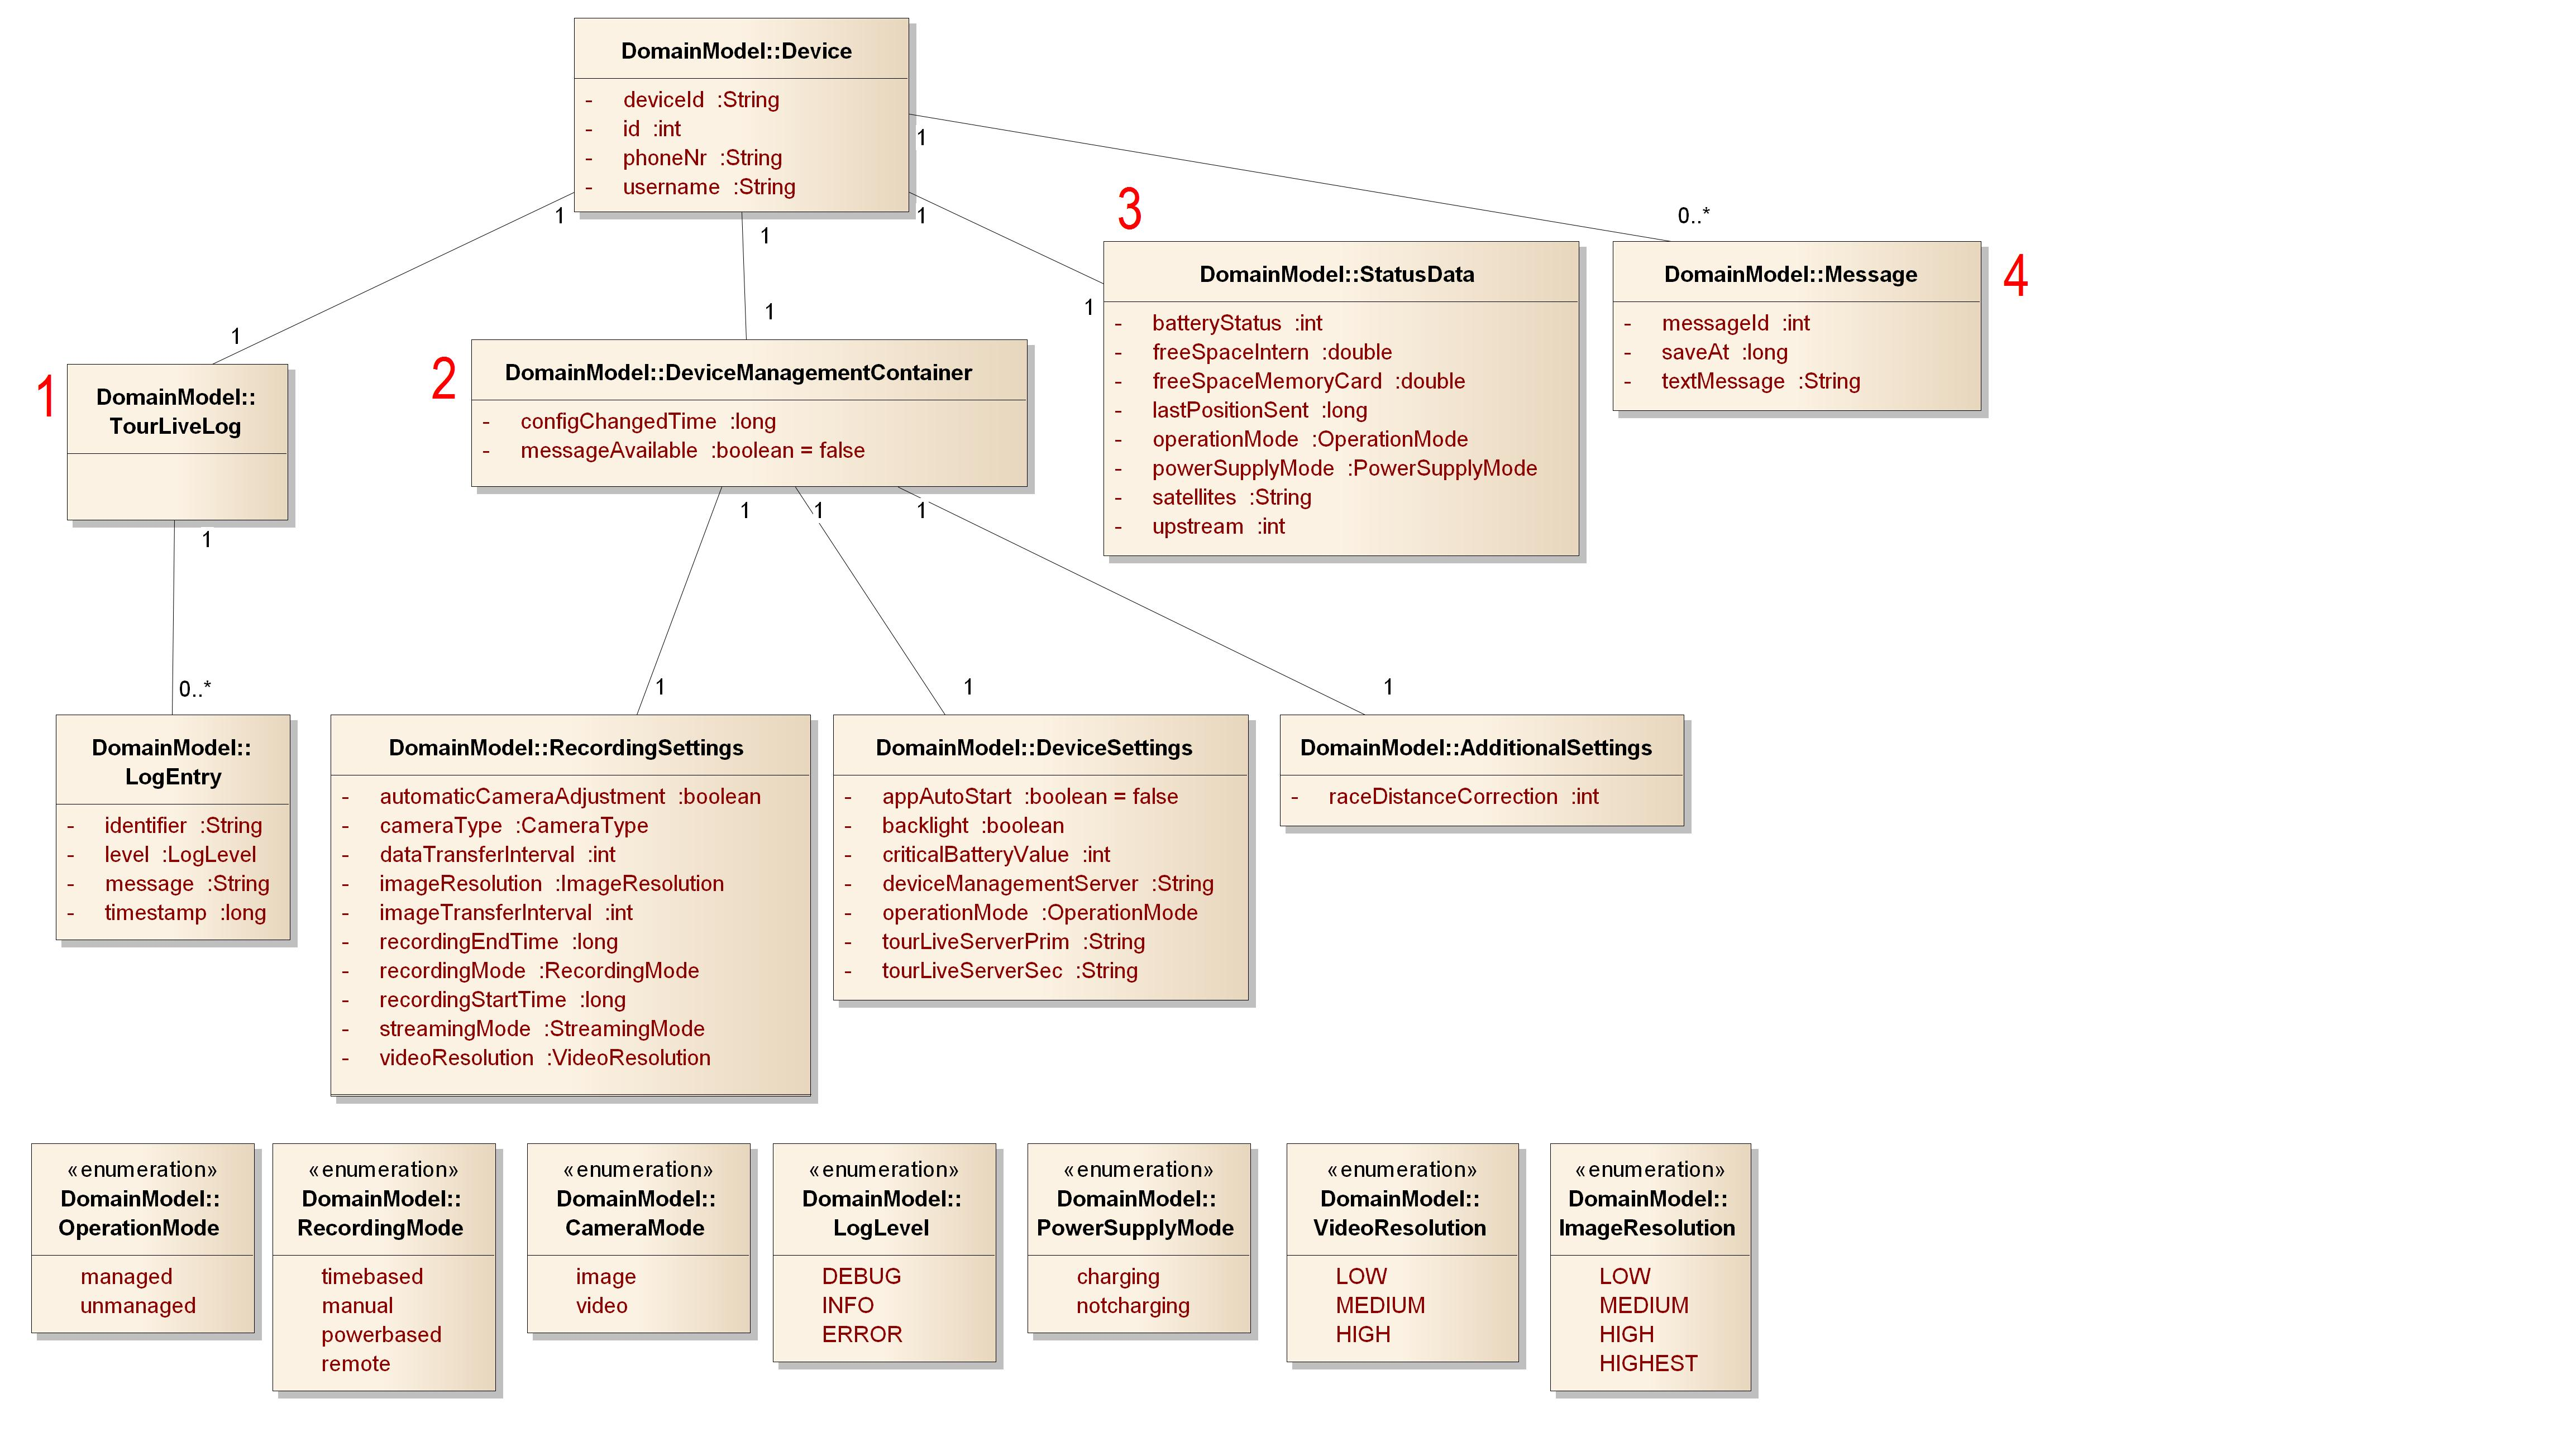
\includegraphics[width=120mm]{images/devmgmtsrv/domainmodel.jpg}
	\caption{Domain Model des Device Management Portals}
\end{figure}


\section{Software Design}
\subsection{Architektur und Übersicht}
Wie auch der TourLive Server hat das Device Management Portal zwei Hauptaufgaben. Zum einen wird die Bearbeitung der Daten ermöglicht und zum anderen wird den Aufnahmesystemen eine API zur Verfügung gestellt.


\begin{figure}[H]
	\centering
	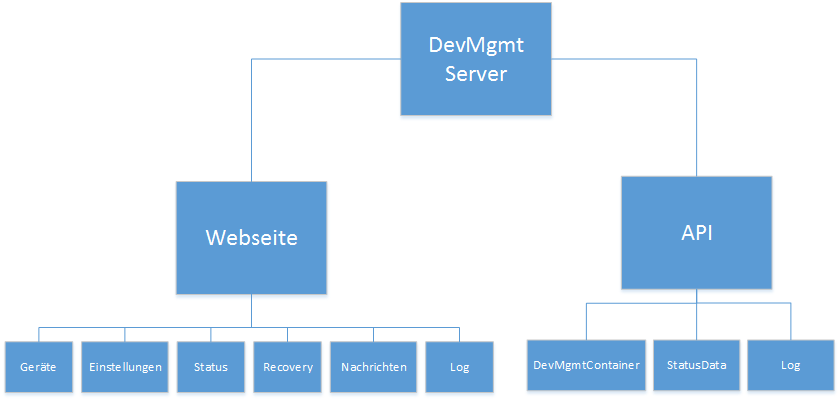
\includegraphics[width=120mm]{images/devmgmtsrv/uebersicht.png}
	\caption{Grobstruktur des Device Management Servers}
\end{figure}

Wie beim TourLive Server besteht dank der gewählten Struktur die Möglichkeit, die Webseite und die API auf verschiedene Server aufzuteilen. Da die Auslastung des DeviceManagement Portals jedoch gering ist, da nur Administratoren darauf zugreifen können, deshalb wird diese Aufteilung nicht weiter erklärt.

\subsection{Schichtenmodell und Paketdiagramm}
Das Device Management Portal ist in vier Schichten unterteilt. Die Schichten wurden an die Struktur des Spring MVC angepasst. In der Abbildung kann man die verschiedenen Schichten mit den jeweiligen Klassen sehen.

\begin{figure}[H]
	\centering
	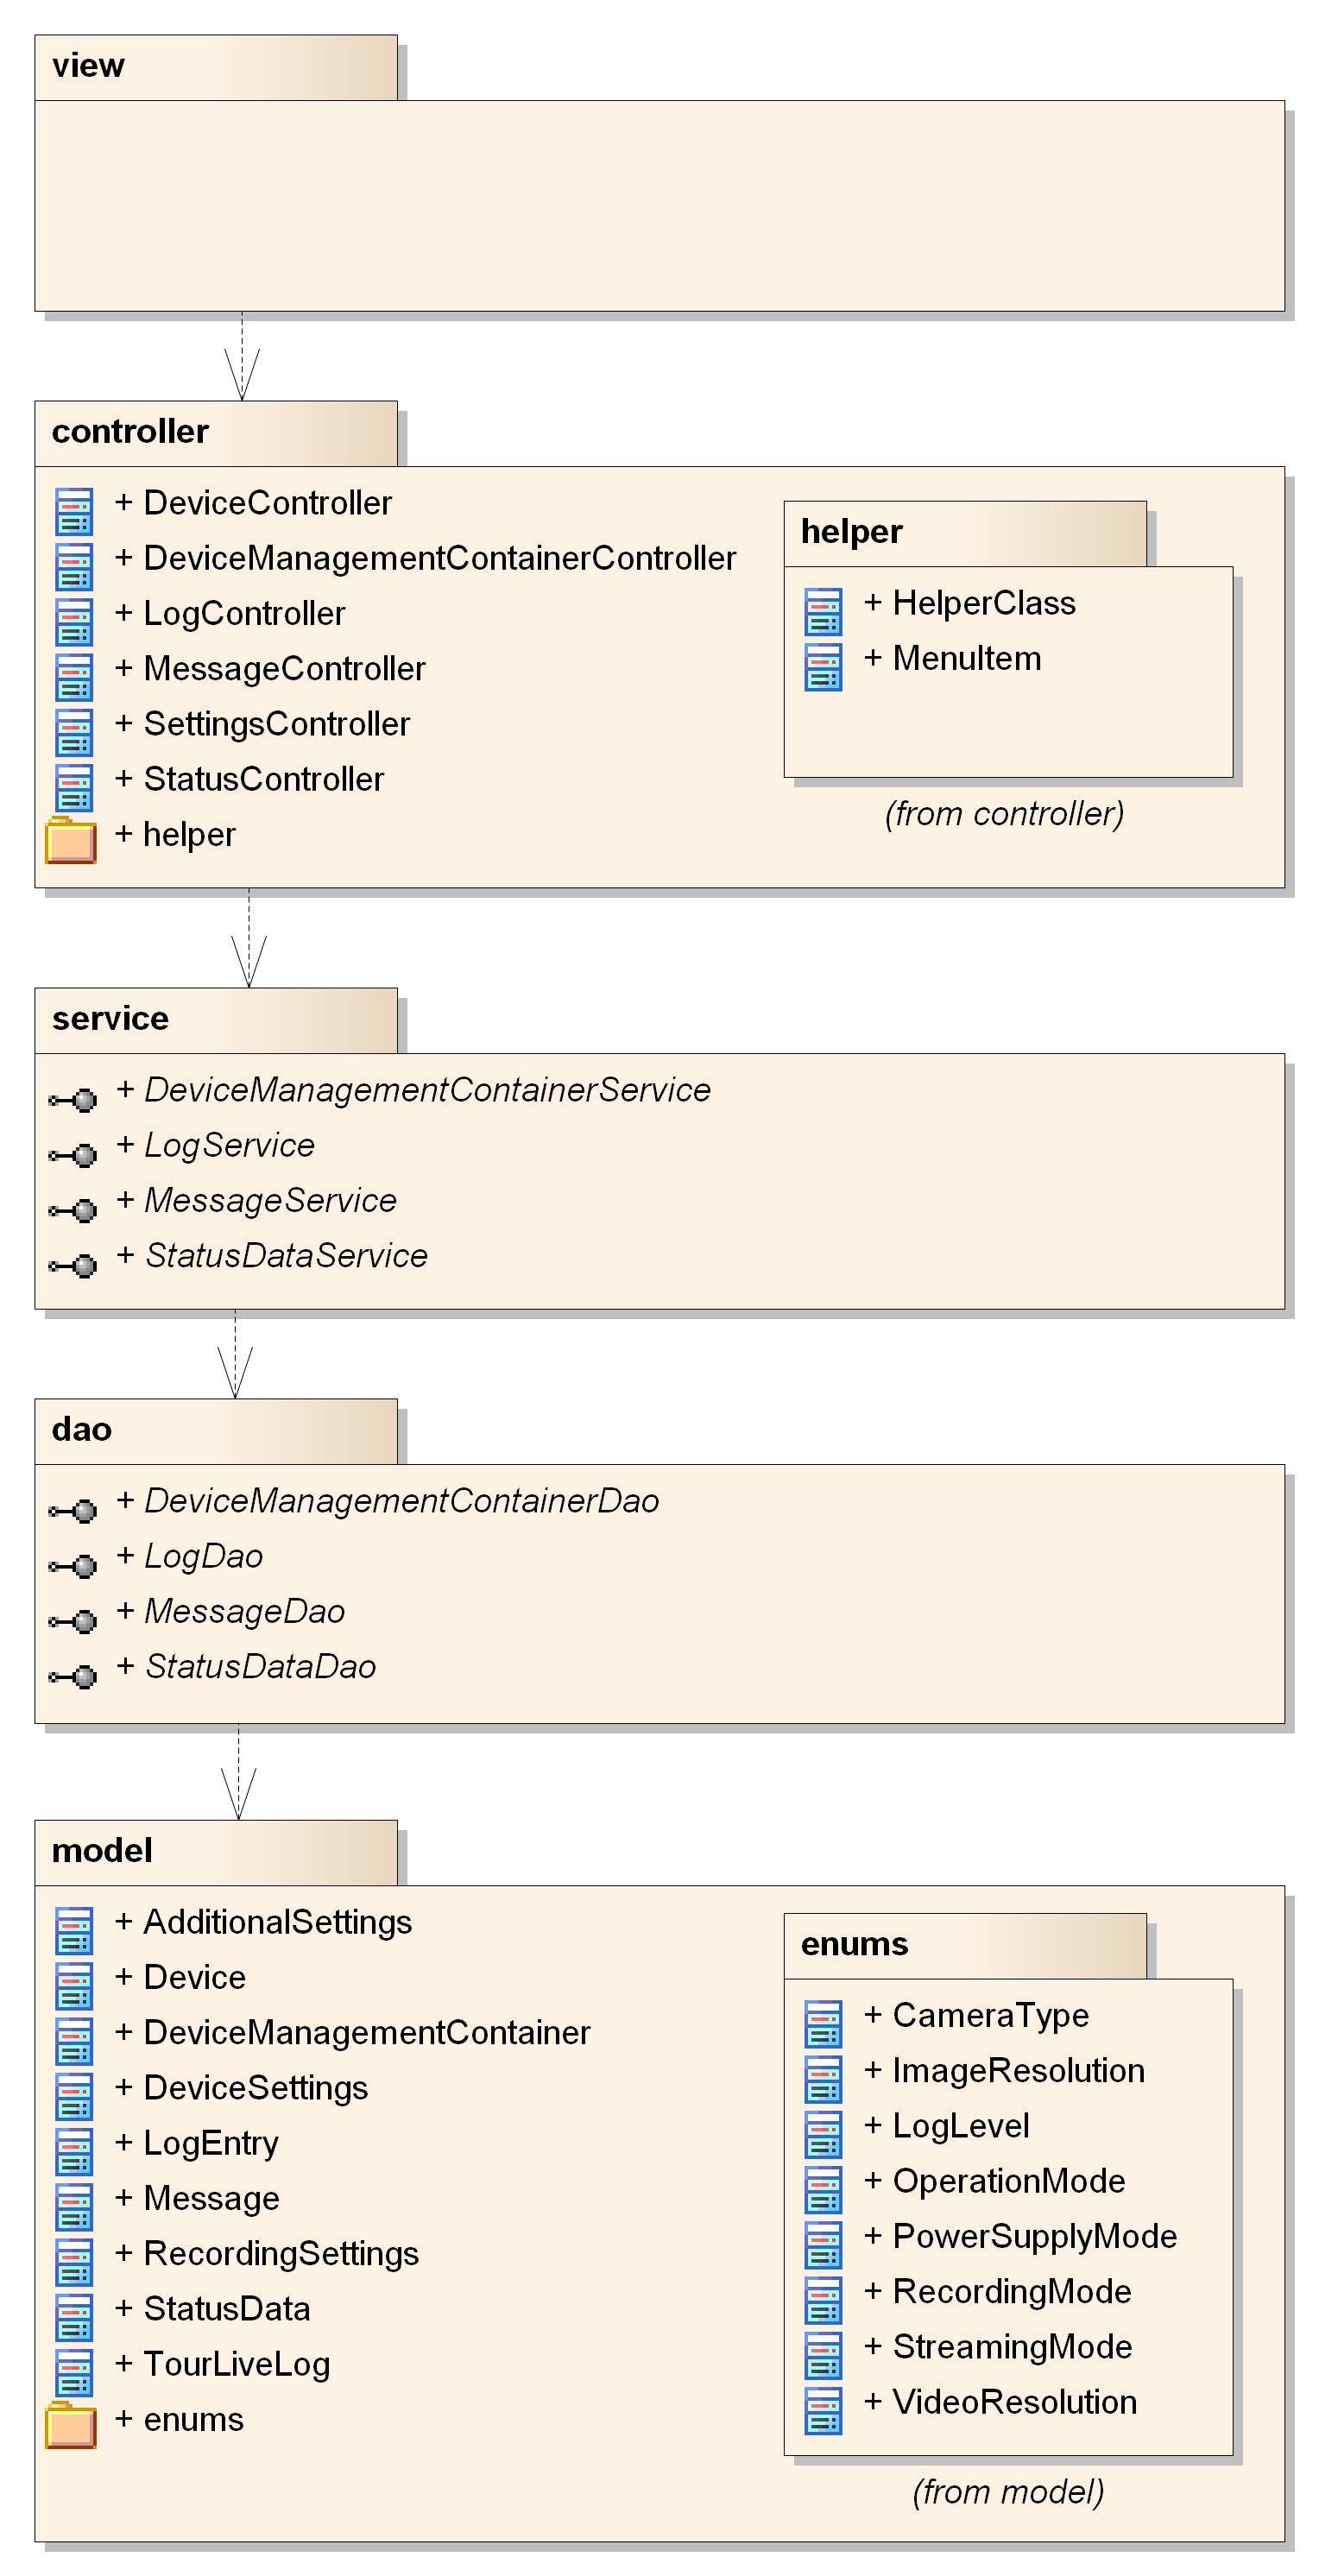
\includegraphics[width=80mm]{images/devmgmtsrv/schichten.jpg}
	\caption{Schichtendiagramm des Device Management Portals}
\end{figure}

\subsubsection{View}
Die View Schicht enthält alle JSP Files, die für die Darstellung benötigt werden. Die Controller stellen den verschiedenen Views die Models zur Verfügung.

\subsubsection{Controller}
Die Controller Schicht stellt die Models für die Anzeige sowie für die API zur Verfügung. In den verschiedenen Controller Klassen werden Attribute gesetzt, um auf die Models zugreifen zu können.

\subsubsection{Service}
Die Service Klassen wissen, wie die Models geladen werden. In unserer Implementation werden die Daten von der Datenbank via Hibernate in die Models geladen.

\paragraph{DeviceManagementContainerService}
Der Device Management Container Service speichert und liefert die Container mit den Einstellungen. Vor dem zurückliefern des Containers wird das Flag \textit{messageAvailable} gesetzt. Zusätzlich managt der Service den Zugriff auf die Geräte. 

\subsubsection{Model}
Die Domäne des Device Management Portals wird in der Model Schicht abgebildet. Für jede Domänenklasse gobt es hier eine Model Klasse. Diese Klassen werden via Hibernate von der Datenbank gespeichert und zurückgeschrieben.

\subsubsection{DAO}
%TODO

\subsection{Device Management Container}
%TODO

\section{Realisierung}
Dieses Kapitel beschreibt die Umsetzung des Device Management Portals.

\subsection{API}
Die API wird mittels Spring Annotations definiert. 

\begin{lstlisting}[language=Java, caption=Spring Annotation]
@RequestMapping(value = "/api/getdevmgmtcontainer", method = RequestMethod.POST)
@ResponseBody
public DeviceManagementContainer getDeviceManagementContainer(@RequestBody final StatusData request)

\end{lstlisting}
\textbf{\textit{@RequestMapping}:} gibt an, welche URL auf diese Methode gemappt wird und welche Request Methode erlaubt ist.\\
\textbf{\textit{@ResponseBody}: } definiert, dass die Methode eine Antwort zurück gibt.\\
\textbf{\textit{@RequestBody}: } der Parameter der Methode wird als Body des Requests definiert.\\
Diese annotierten Methoden müssen in einer Klasse enthalten sein, welche als \textit{@Controller} annotiert ist.


\subsection{Webseite}
Die Webseiten wurden mit JSP umgesetzt. Als Erweiterung wurde Javascript sowie das JQuery Plugin verwendet. Um die grafische Oberfläche möglichst einfach zu gestalten, wurde das Twitter Bootstrap \footnote{Twitter Bootstrap, \url{http://twitter.github.io/bootstrap/}, besucht am 25. Mai 2013} CSS benutzt.

Die Webseite wird in drei Teile unterteilt, Header, Footer sowie der Hauptbereich. 

\begin{figure}[H]
	\centering
	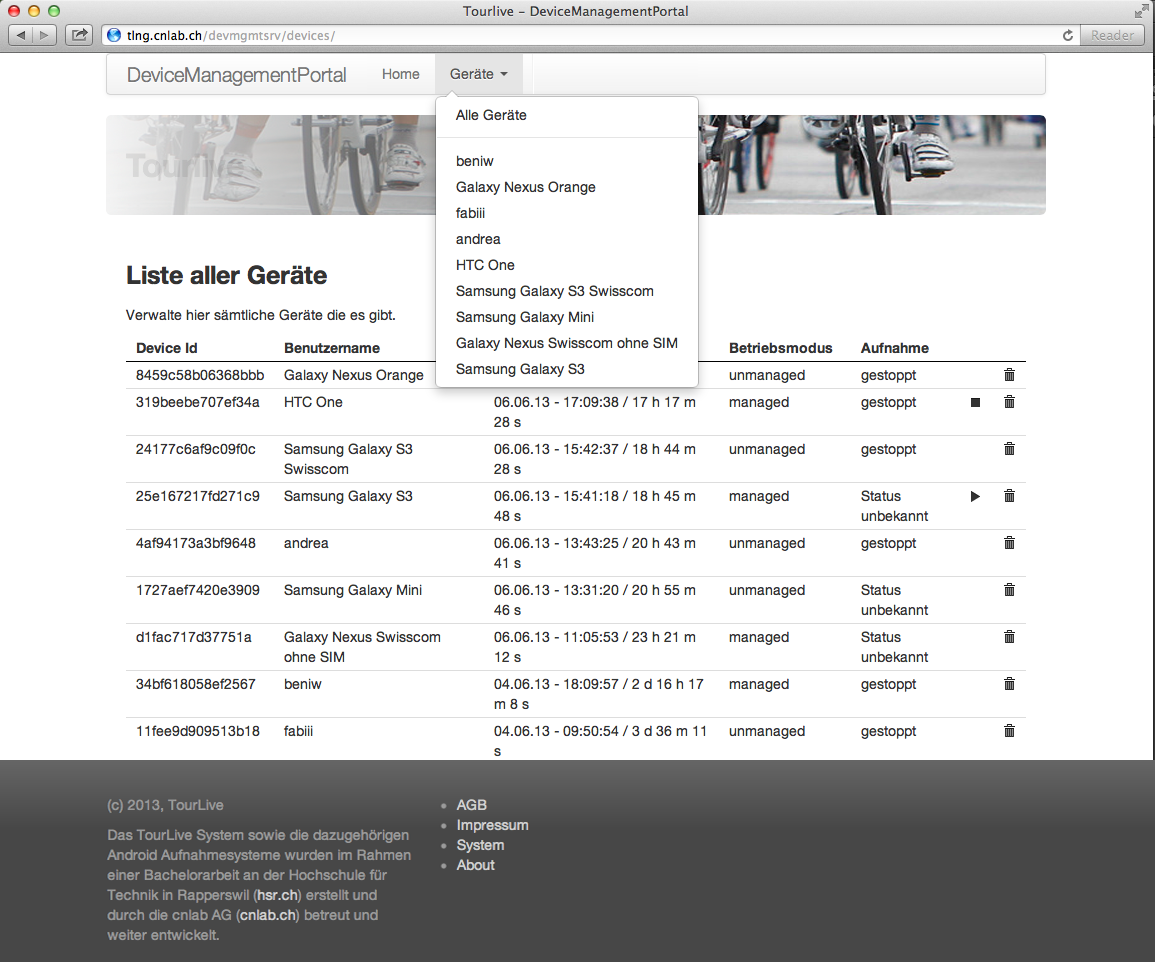
\includegraphics[width=120mm]{images/devmgmtsrv/all.png}
	\caption{Übersicht der DevMgmt Webseite}
\end{figure}

\subsubsection{Header}
Im Header hat man die Möglichkeit, über eine Schnellnavigation auf ein Gerät zuzugreifen. 
\begin{figure}[H]
	\centering
	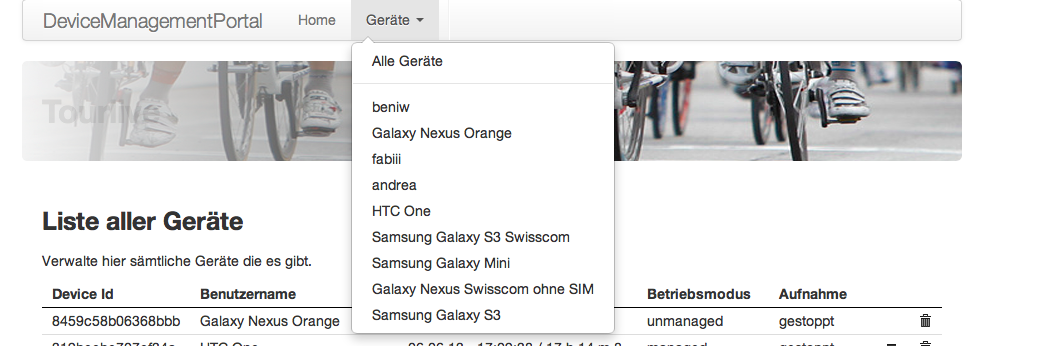
\includegraphics[width=120mm]{images/devmgmtsrv/header.png}
	\caption{DevMgmt Webseite Header}
\end{figure}



\subsubsection{Footer}
Der Footer enthält detaillierte Informationen zum Projekt TourLive. 
 
\begin{figure}[H]
	\centering
	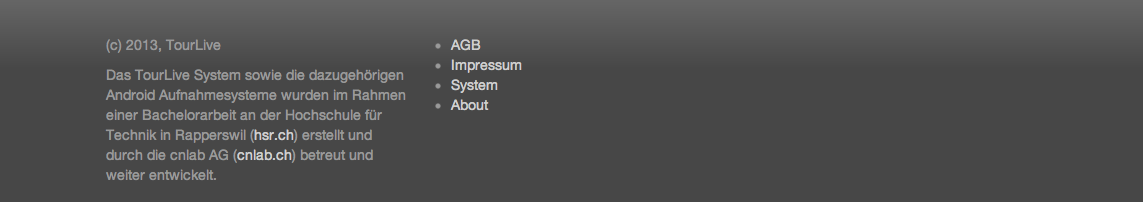
\includegraphics[width=120mm]{images/devmgmtsrv/footer.png}
	\caption{DevMgmt Webseite Footer}
\end{figure}


\subsubsection{Hauptbereich}
Der Hauptbereich unterteilt sich wieder in zwei Teile. So hat man Links eine neue Navigation, mit welcher man sich zwischen den verschiedenen Seiten hin und her bewegen kann. 
 
\begin{figure}[H]
	\centering
	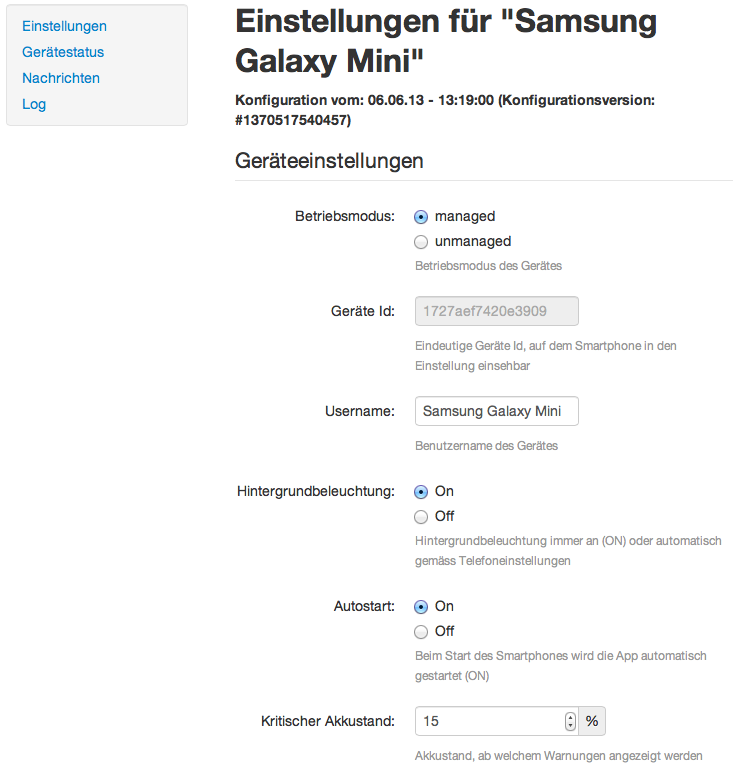
\includegraphics[width=120mm]{images/devmgmtsrv/settings.png}
	\caption{DevMgmt Webseite Hauptbereich}
\end{figure}

\subsection{Datenbank}
Die Speicherung der Daten in der Datenbank erfolgt mittels Hibernate automatisch. 
